\documentclass{article}
\usepackage{bnaic}
\usepackage{url}
\usepackage{graphicx}
\usepackage[section]{placeins}


%% if your are not using LaTeX2e use instead
%% \documentstyle[bnaic]{article}

%% begin document with title, author and affiliations

\title{\textbf{\huge Traffic Control Simulation - Report v.2}}
\author{Elbert Fliek (s1917188) \affila \and
    Albert Thie (s1652184) \affila \and
    No\"el L\"uneburg (s1773135) \affila}
\date{\affila\ \textit{University of Groningen \\
\today}}

\pagestyle{empty}

\begin{document}
\ttl
\thispagestyle{empty}

\begin{abstract}
    Improving the amount of thoroughfare at crossroads using traffic lights has been a topic of research in urban planning and traffic engineering. Multiple systems have been designed to increase traffic flow in intersections using sensors in traffic lights and optimization based on traffic data. Our research shows the advantage of applying a state of art sorting algorithm and combining this with information about the traveling direction of individual cars. Thus taking advantage of communicating traffic lights and individual cars, we hope to improve traffic flow in intersections. Results show that vehicles are able to continue onto the intersection without stopping more often when simulating a smart traffic control system.
\end{abstract}

%\begin{abstract}
%\noindent
%\end{abstract}


\section{Introduction}
\subsection{The problem}
Optimizing the traffic flow is a problem which has been studied with computational models in a variety of ways. One possible approach is modelling the behavior of traffic by using natural laws, such as those governing the expansions and transfer of kinetic gas \cite{helbing2001master}. This however, does not solve the problem of optimizing the traffic lights at an intersection. To increase the amount of traffic that can pass an intersection, and reduce the wait time at the intersection, other models are needed.

\subsection{State of the Art}
According to Li et. al \cite{survey2014} the problem of intersection management can be tackled with a combination of not only optimizing the sorting algorithm that schedules green lights based on queue length, but also using predictions of future traffic reaching the intersection. These predictions can be based on data gathered over time at an intersection, thus identifying times of heavy traffic. Their overview however only identifies possible approaches to the problem and not an actual implementation that can be simulated.

L{\"a}mmer et al. \cite{self_control2008} however created a simulation based on fluid dynamics.  L{\"a}mmer et. al. view the problem of intersections as a multi-agent problem, where both traffic lights and individual vehicles interact together. Traffic lights assign priority among each other by detecting not only waiting traffic, but also oncoming traffic. Oncoming traffic indicates its current speed and project trajectory, allowing traffic lights to take this into account when deciding priority among themselves. This allows for platoon of oncoming vehicles to influence decision making in a traffic light. Through the pressure of "future"  cars, the green wave effect for a platoon of cars can be created emergently.

This approach was tested not only in traffic simulations, but also implemented in two real life intersections in the city of Dresden \cite{site}. The real life application notably increased traffic flow and allowed for preferential treatment for public transport vehicles, further helping the city's infrastructure.


\subsection{New Idea}
L{\"a}mmer et al have a simple experimental setup. All vehicles are the same, and no vehicles make a turn. We aim to test if there hypothesis also holds when we simulate a situation that has cars with different specifications and the ability to make a turn at the intersection.

We expect L{\"a}mmer's system to also work in this, more lifelike, situation, but feel it must nonetheless be researched.



\section{Method}
The dynamic queue by L{\"a}mmer et. al. is compared to regular traffic control systems in a simulation environment. Both systems use a four square intersections with vehicles approaching at random intervals from all sides. Intervals are increased and decreased to measure the effects of high and low traffic flow situations. 

Time in the simulation is measured in frames, while individual of vehicles is measured in traversed pixels. This abstraction allows for vehicles speed, brake and acceleration time to be measured in screen movement.

The regular traffic system uses a fixed minimum green time for each traffic light. After this time expires, each lane is checked for total number of cars stopped in front of the intersection, emulating road sensors. The lane with the highest number of cars is then given the minimum green time.

The dynamic system uses a queue based approach, where the amount of vehicles in the queue determines not only which light will be green next, but also the time the light will remain green. Green time is decided by the amount of present and approaching cars in the queue, the amount of start up time needed for cars to start moving and the time needed to clear the intersection after all cars have left. 


\subsection{Simulation environment}
We have developed an environment that allows simulation of traffic on intersections. Traffic light status and vehicle activity is visualized from a top-down view.

A simulated traffic scenario contains an intersection with lanes going towards and away from it. A variety of vehicles occupy these lanes. This section describes properties that can be adjusted for each entity.

See figure 1 for a screenshot of the test setup.

\begin{figure}[h!]
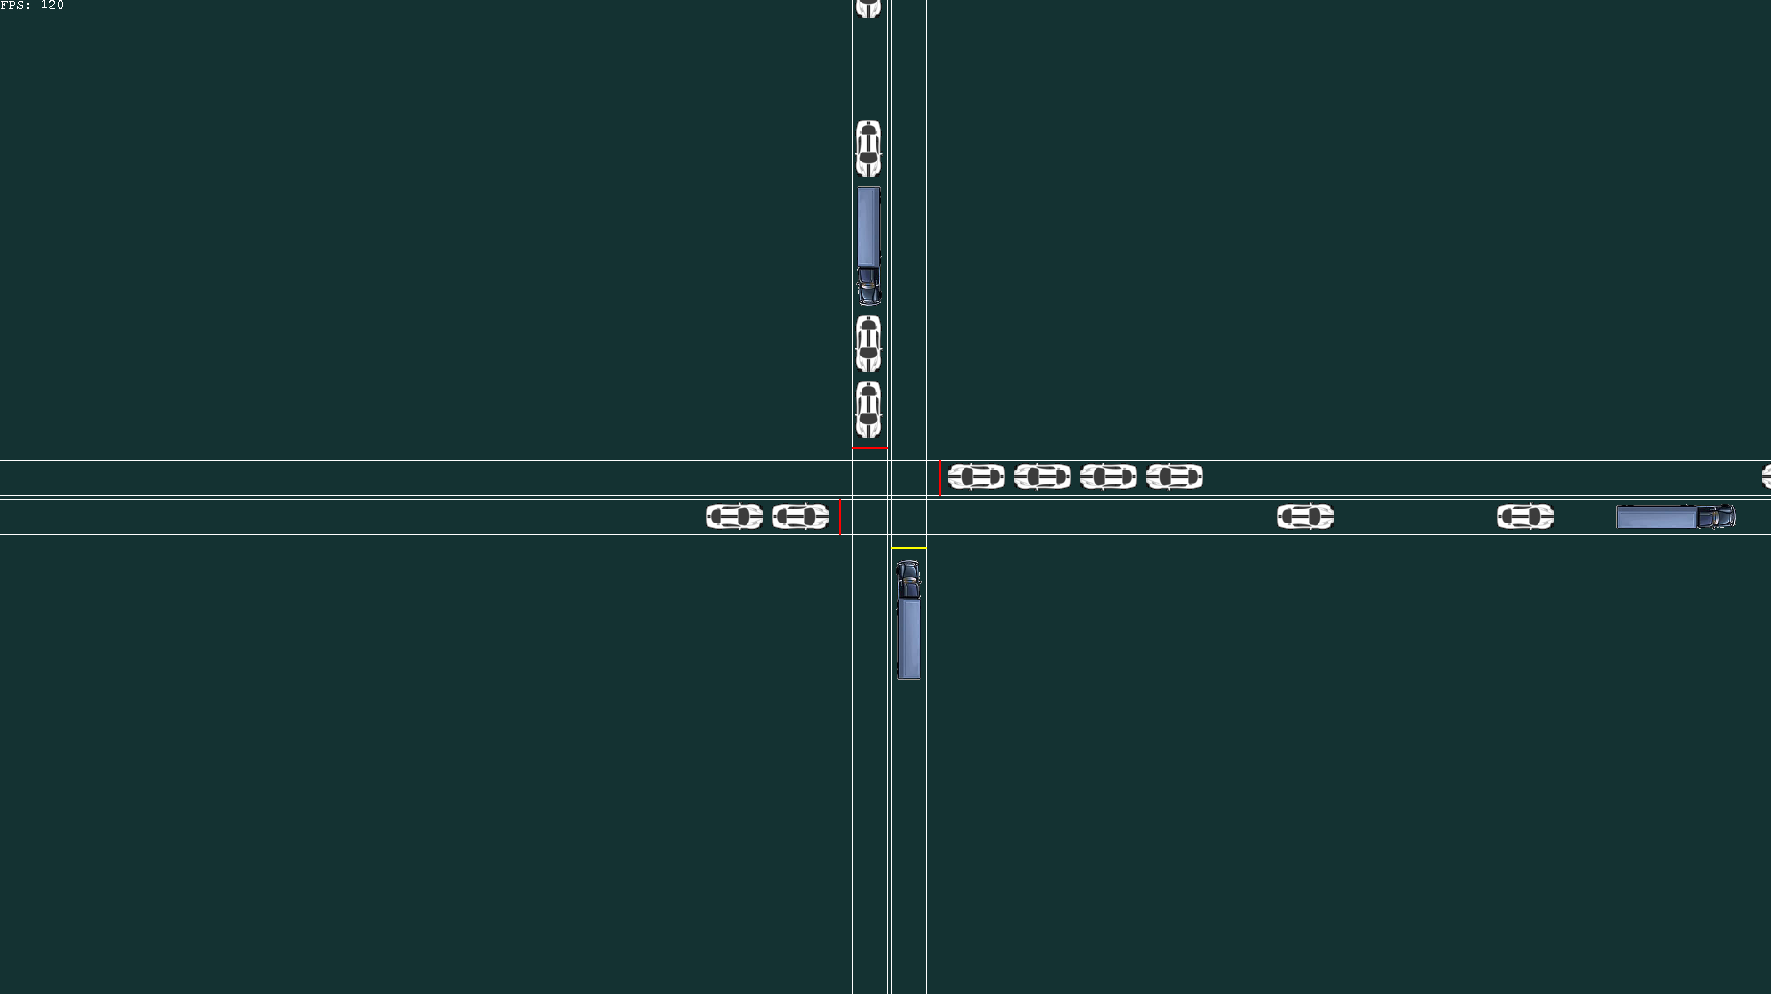
\includegraphics[width=12cm]{sim_screenshot.png}
\caption{A screenshot of the simulation}
\end{figure}

\paragraph{Simulation} ~\\
The simulation framework includes the following parameters: \\
\textbf{Spawn frequency} ~ The rate at which vehicles are added randomly to an arbitrary lane going towards the intersection.\\
\textbf{Safety distance} ~ Distance maintained between vehicles in a queue to prevent collisions.\\
\textbf{Communication distance} ~ Maximum distance below which incoming vehicles can communicate with the traffic lights.

\paragraph{Intersection} ~\\
An intersection within our simulation can connect roads in up to four directions; north, south, east and west. \\
\textbf{Number of lanes} ~ The number of lanes in each direction is used to modify traffic capacity and affect the complexity of the traffic situation.\\
\textbf{Traffic lights} ~ Traffic lights can be placed on lanes entering the intersection, signalling whether or not approaching vehicles can proceed.

\paragraph{Vehicle} ~\\
Each vehicle is tied to a lane heading toward or away from an intersection. Vehicles are individual agents with the following properties:\\
\textbf{Length} ~ Length of the vehicle.\\
\textbf{Turning rate} ~ Duration for this vehicle to fully turn either right or left on an intersection.\\
\textbf{Deceleration} ~ Braking constant, determines the rate at which the speed diminishes when a vehicle is slowing down.\\
\textbf{Acceleration} ~ Acceleration constant, determines the rate at which the speed increases when a vehicle accelerates.\\
\textbf{Maximum speed} ~ Maximum speed of the vehicle.\\

\subsection{Experimental setup}
\label{exp_setup}
Two traffic control systems are compared. The first is a regular system which operates based on inputs from road sensors in front of traffic lights. Each vehicle that passes one of these sensors generates a pulse. The total number of pulses determines the priority of the lane going into the intersection. The lane with the highest current priority will show a green signal, but only after every other lane has shown a red signal. This entails that only one lane can be active at one time. To avoid rapid light changes, a minimum green signal duration is enforced.

The second system is similar in that it operates using a lane priority system. However, more information is available, such as the type of each vehicle, and traffic density in a particular direction. Each traffic signal has access to traffic information of the lane that it is assigned to. Communication between traffic signals of different lanes determines which lane is allowed access to the intersection at any point in time.

To quantify the performance of both systems we measure the average waiting time of all vehicles.

\section{Results}
Figure 2 shows the distribution of wait times at the traffic light under the default traffic control system. The peak at wait time 0 indicates situations in which a vehicle was able to pass through a green light without having to stop.

Figure 3 shows the distribution of wait times at traffic lights under the system designed by L{\"a}mmer et al. There is a large peak at the 0 frame wait time, with no secondary peaks. This distribution has a slightly longer tail compared to the default method, indicating that some cars had to wait longer than any car in the default traffic control situation.
\begin{figure}[h!]
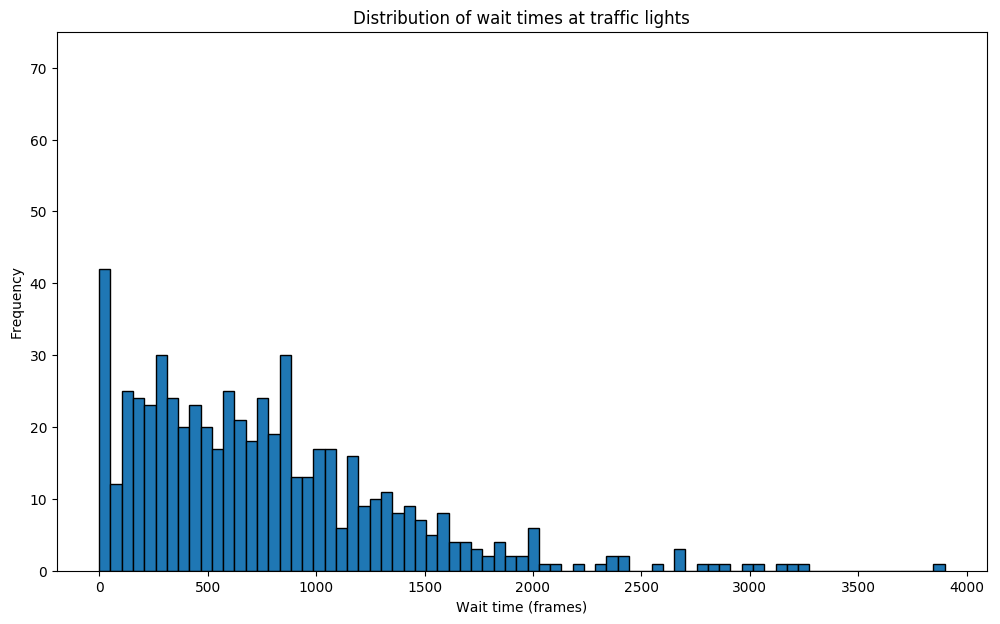
\includegraphics[width=12cm]{img/default_1wait_time.png}
\caption{Distribution of wait times at the traffic light under the standard traffic control system}
\end{figure}
\begin{figure}[h!]
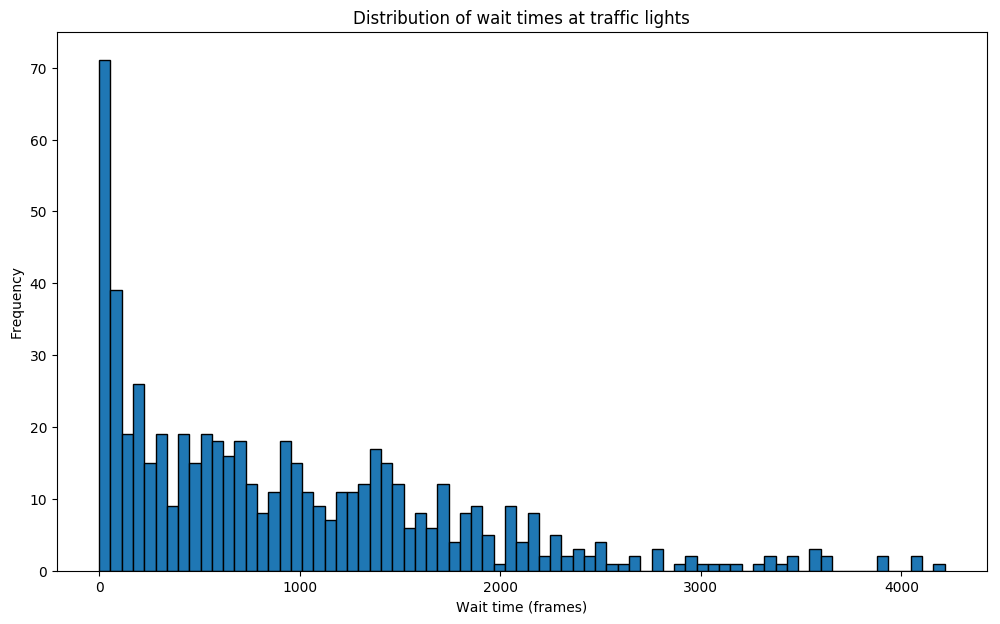
\includegraphics[width=12cm]{img/Laemmer_1wait_time.png}
\caption{Distribution of wait times at the traffic light under the L{\"a}mmer traffic control system}
\end{figure}

\FloatBarrier

\section{Conclusion}
As the results show, our findings are partially in line with the findings of L{\"a}mmer et al. The smart traffic system allows cars to pass through the intersection without having to stop more frequently than a more trivial approach.

The second observation we can make from the results is that there is one significant downside to the L{\"a}mmer traffic control system, some people will have to wait longer than in the simpler traffic control system. This is because any light will attempt to fully clear its lane, including incoming cars. In turn, other lanes will have to wait longer.

We can conclude that our simulation shows no significant difference in wait times between the method of L\"{a}mmer and our default method, as a trade-off is created between longer green times to fully clear lanes and longer wait times for lanes with a red light at the same time. We feel L\"{a}mmer's method would be more suitable to an intersection with imbalanced lanes with regards to traffic density.


\section{Additional lessons learned}
After a considerable amount of time was spent during the development of our own simulation, built from scratch, we came across a toolkit that was specifically designed to test traffic engineering solutions (PTV Vistro). In hindsight using that toolkit would have been considerably easier.

\bibliographystyle{plain}
\bibliography{literature}



\end{document}


